\clearpage
\subsubsection{Modificación de parámetros internos del modelo, parámetros de entrenamiento, parámetros de generación de mezclas, de efectos y de la formación de transformadas de Fourier}

Existe además una sección de la interfaz que permite modificar los parámetros de formación de las transformadas de Fourier y los parámetros internos del modelo, ver Figura \ref{fig:params-stft-gui}. Estos parámetros son intrínsecos al modelo y afectan a la separación de fuentes.

\begin{figure}[H]
    \centering
    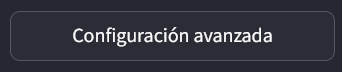
\includegraphics[width=\textwidth,height=0.16\textheight,keepaspectratio]{commons/BotonConfig_GUI.png}
    \caption{Botón de configuración.}
    \label{fig:boton-config-gui-1}
\end{figure}

El sistema lleva a la persona usuaria a una nueva pantalla donde se pueden modificar variedad de parámetros, ver Figura \ref{fig:params-completos-gui}. 

Entre los parámetros que permite modificar el sistema a la persona usuaria están: los de formación de las transformadas de Fourier, ver Figura \ref{fig:params-stft-gui}. Además, se pueden modificar los parámetros de entrenamiento de nuevos modelos, ver Figura \ref{fig:params-train-gui}, los parámetros de generación de efectos, ver Figura \ref{fig:params-efectos-gui}, y los parámetros de generación de mezclas, ver Figura \ref{fig:params-generacion-gui}.

\begin{figure}[H]
    \centering
    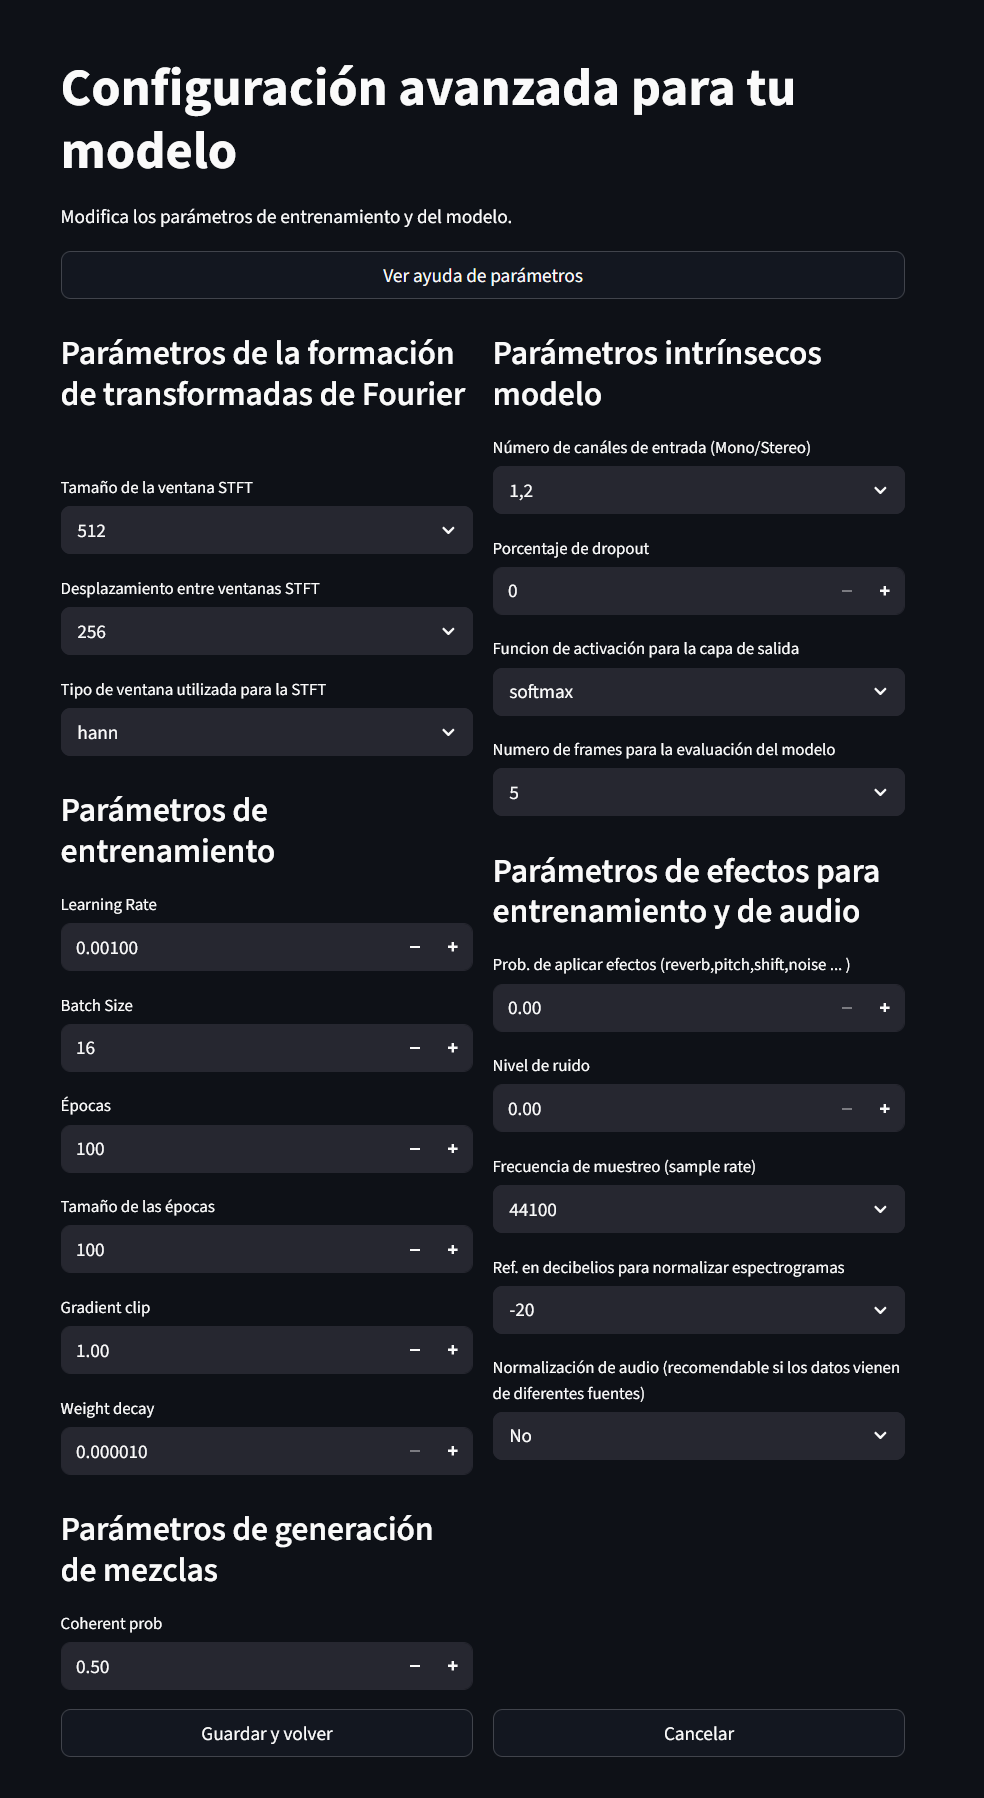
\includegraphics[width=0.7\textwidth]{commons/config-avanzada-completa-GUI.png}
    \caption{Parámetros de formación de transformadas de Fourier modificables en la interfaz visual.}
    \label{fig:params-completos-gui}
\end{figure}

\begin{figure}[H]
    \centering
    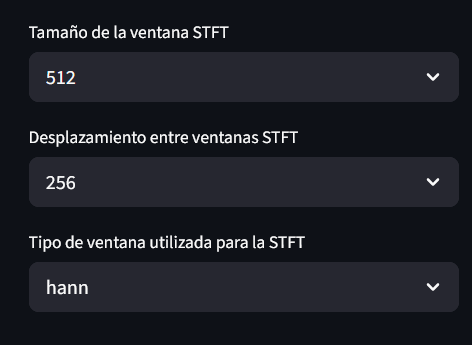
\includegraphics[width=\textwidth,height=0.16\textheight,keepaspectratio]{commons/ParamsSTFT_GUI.png}
    \caption{Parámetros de formación de las transformadas de Fourier modificables en la interfaz visual.}
    \label{fig:params-stft-gui}
\end{figure}

\begin{figure}[H]
    \centering
    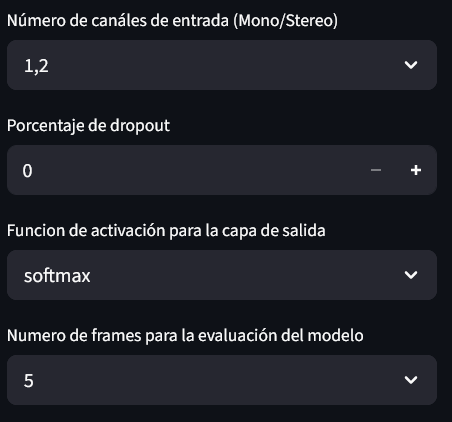
\includegraphics[width=\textwidth,height=0.16\textheight,keepaspectratio]{commons/ParamsModelo_GUI.png}
    \caption{Parámetros intrínsecos del modelo modificables en la interfaz visual.}
    \label{fig:params-modelo-gui}
\end{figure}

\begin{figure}[H]
    \centering
    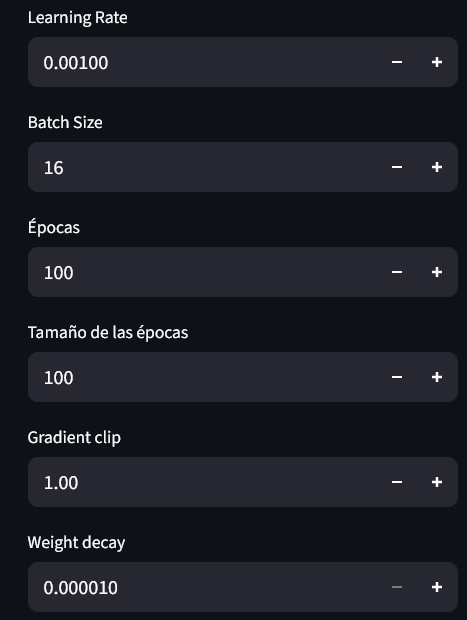
\includegraphics[width=\textwidth,height=0.16\textheight,keepaspectratio]{commons/ParamsEntrenamiento_GUI.png}
    \caption{Parámetros modificables de entrenamiento de nuevos modelos en la interfaz visual.}
    \label{fig:params-train-gui}
\end{figure}

\begin{figure}[H]
    \centering
    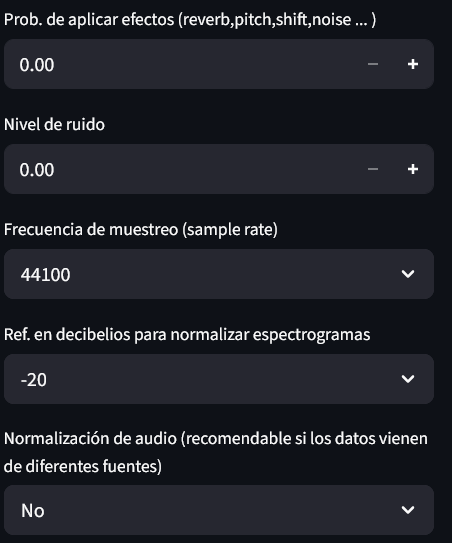
\includegraphics[width=\textwidth,height=0.16\textheight,keepaspectratio]{commons/ParamsEfectos_GUI.png}
    \caption{Parámetros modificables de generación de efectos en la interfaz visual.}
    \label{fig:params-efectos-gui}
\end{figure}

\begin{figure}[H]
    \centering
    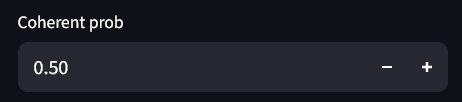
\includegraphics[width=\textwidth,height=0.16\textheight,keepaspectratio]{commons/ParamsMezclas_GUI.png}
    \caption{Parámetros modificables de generación de mezclas en la interfaz visual.}
    \label{fig:params-generacion-gui}
\end{figure}